\documentclass[main.tex]{subfiles}
\begin{document}
    \chapter{Next Steps}
    \label{ch:next-steps}
    We have split this competition year broadly into three "phases," corresponding to the University of Waterloo's academic terms.
    
    \section{Design Phase, Aug 2017 - Jan 12, 2018}
    We outline the accomplishments during this phase in \hyperref[ch:intro]{the Introduction}.
    
    \section{Build Phase, Jan 2018 - Apr 2018}
    The second phase, the Build Phase, starts directly after the FDP submission; the plan is to have functioning and well-tested separate subsystems by April. Additionally, we have set a goal of \$100,000 in sponsorship from companies in Canada and outside, leaving room for unplanned technical expenses. We think this goal will be relatively easy to reach, allowing us to put additional resources toward side projects such as building a several-hundred-foot test track, investigating a Linear Induction Motor design for Competition 4, and building a stronger outreach program. (\hyperref[app:bom]{Appendix \ref{app:bom}} on page \pageref{app:bom} provides cost estimates of all the components of the pod.)
    
	\section{Test Phase, May 2018 and onwards}
    The third phase, the Test Phase, will primarily be the full assembly of the pod and performing all full-pod tests. As we don't know the exact date of the next Hyperloop Competition, we're not able to plan this in too much detail. However, if the competition is in August again, we are planning to complete all the checklists and inspections outlined in the Safety and Testing Checklist ourselves before setting foot in California.
    
    \section{Pod Production Schedule}
    A rough Pod Production Schedule follows; this will be refined as details about the competition date and external factors such as part lead times and sponsorship bottlenecks become more clear.
    
    \begin{figure}
        \centering
        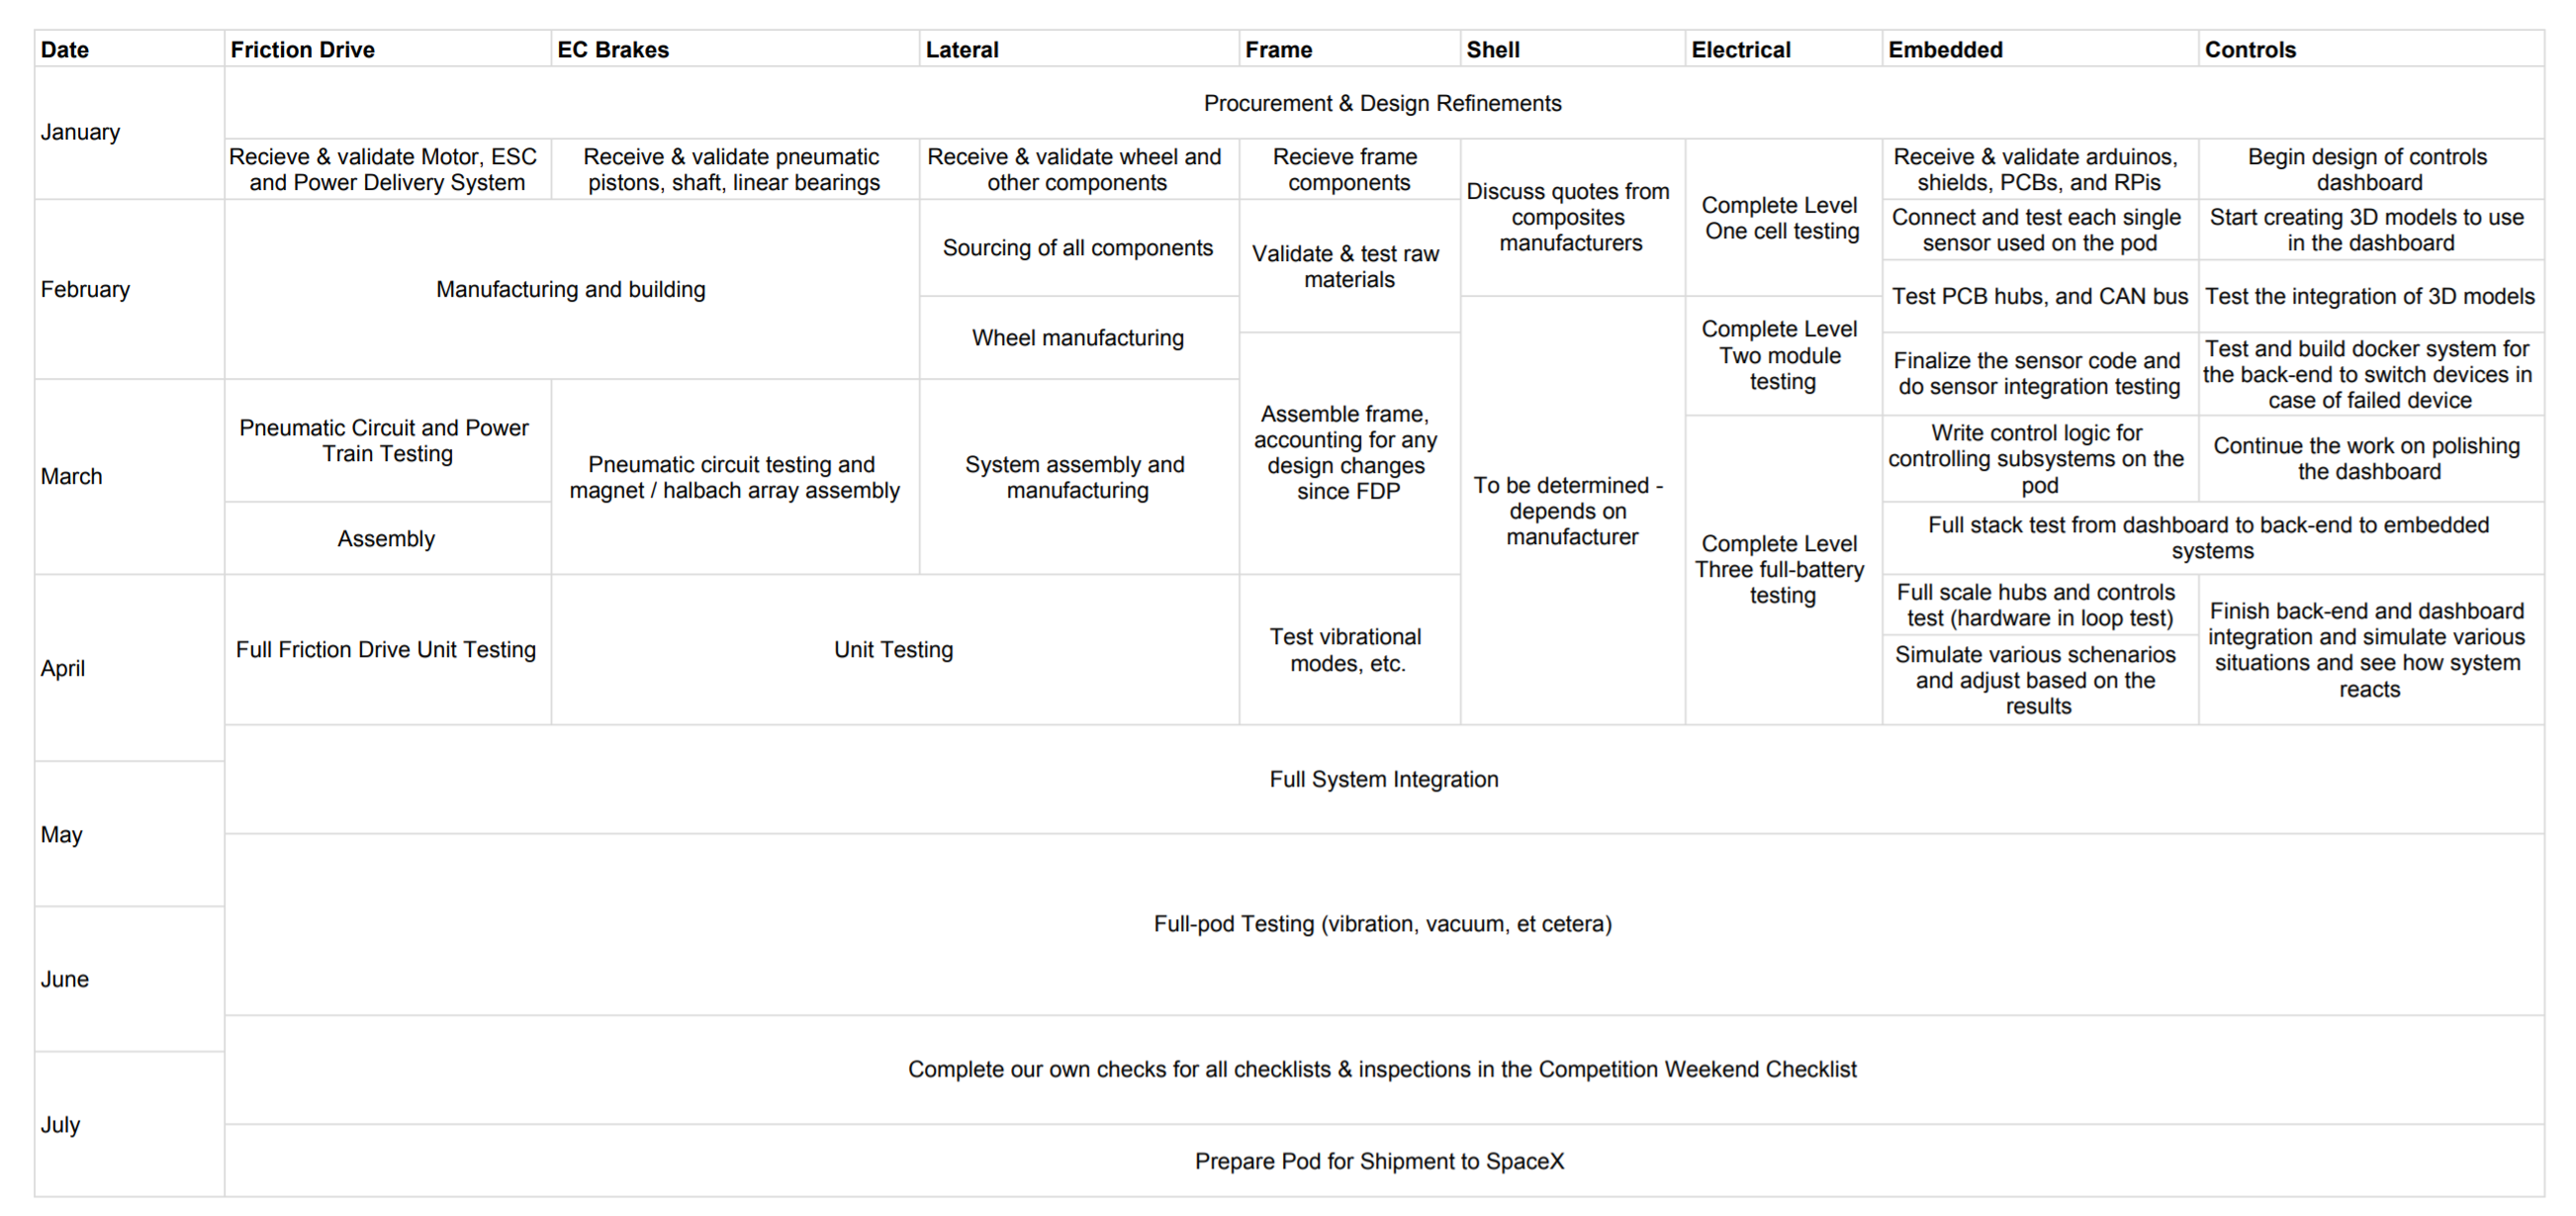
\includegraphics[width=\textwidth]{images/productionsched.png}
        \label{fig:pps}
    \end{figure}

\end{document}
